\section{Wyniki pracy}

%------------------------------------------------

\begin{frame}
    \frametitle{Uruchomienie symulatorów}
    \begin{figure}
        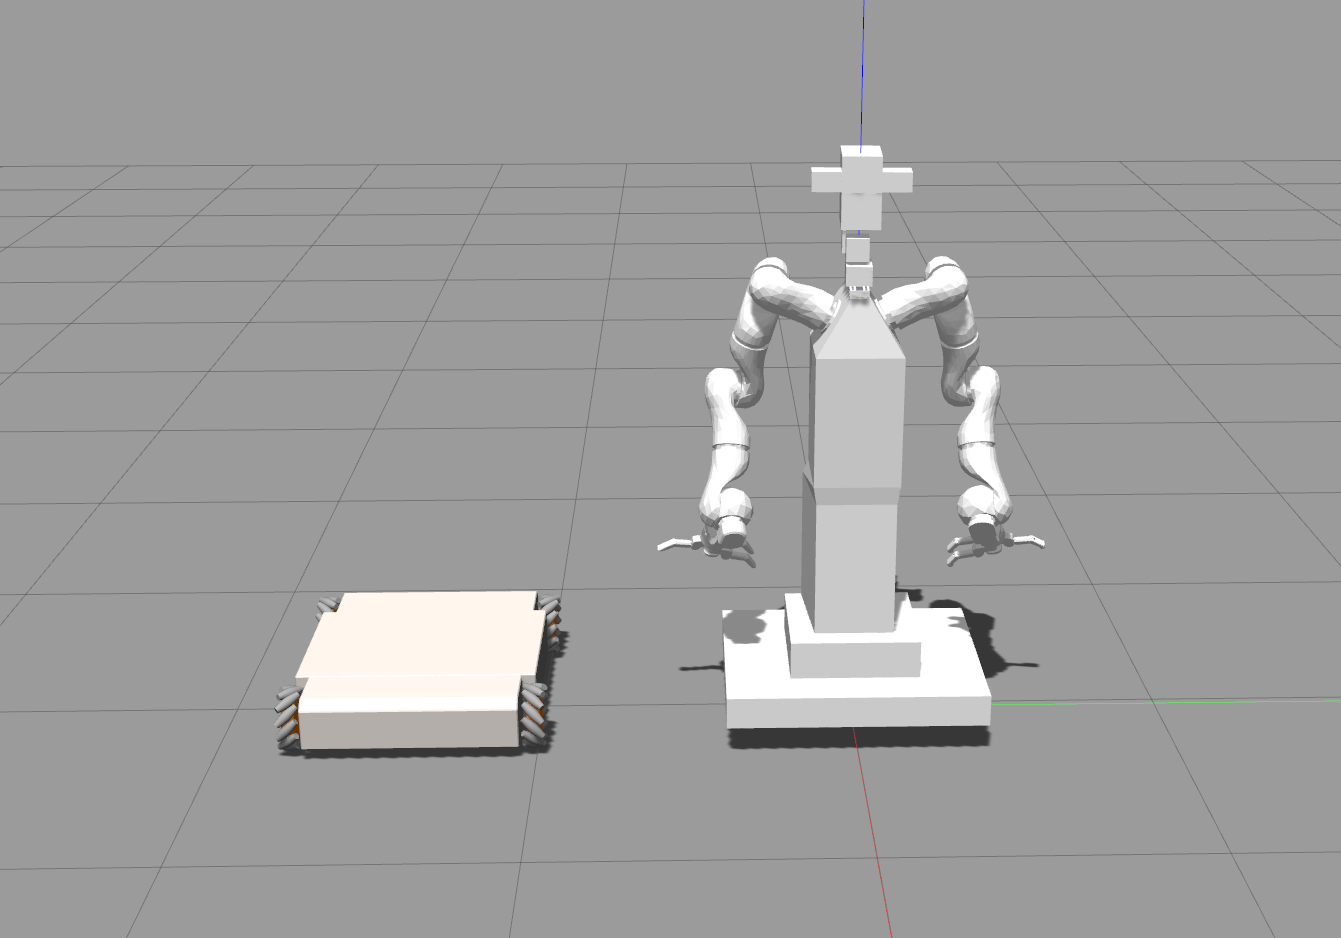
\includegraphics[scale=0.20]{./images/velma+omnivelma_cropped.png}
        \caption{Modele korpusu i bazy mobilnej w jednym świecie symulacji}
    \end{figure}
\end{frame}

%------------------------------------------------

\begin{frame}
    \frametitle{Unifikacja modeli}
    \begin{figure}
        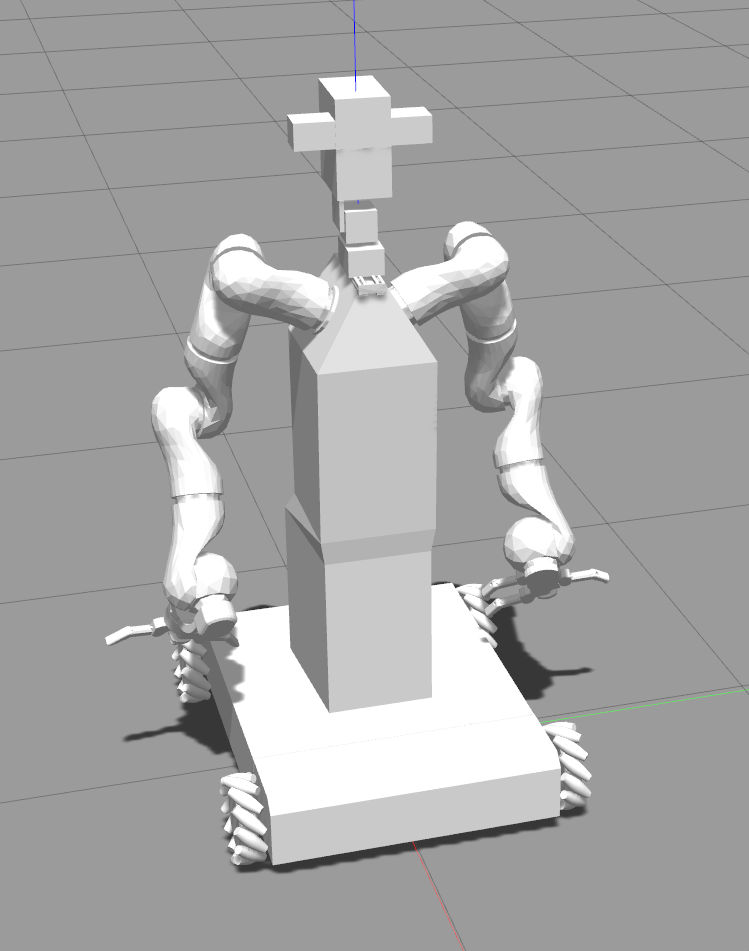
\includegraphics[scale=0.27]{./images/omnivelmomobil-cropped.png}
        \caption{Wstępnie połączone modele korpusu i bazy mobilnej (bez czujników)}
    \end{figure}
\end{frame}

%------------------------------------------------

\begin{frame}
    \frametitle{Proste zadanie manipulacji}
    \begin{figure}
        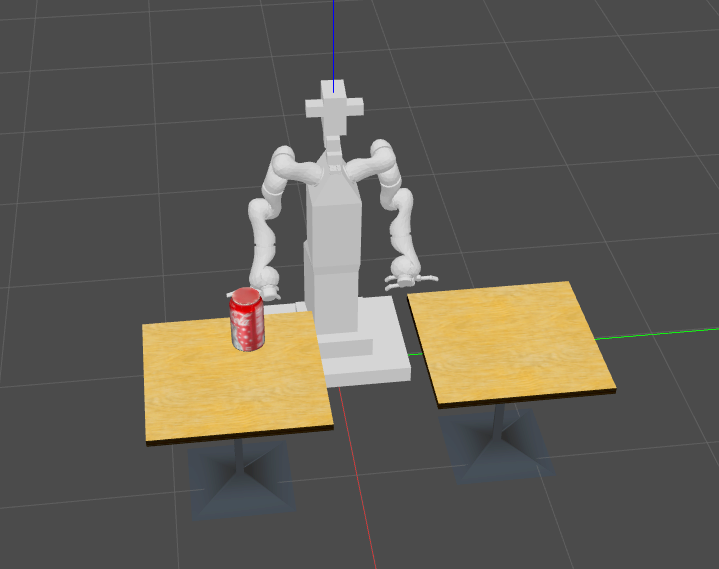
\includegraphics[scale=0.35]{./images/velma_stero_task.png}
        \caption{Zadanie przenoszenia puszki ze stolika na stolik}
    \end{figure}
\end{frame}

%------------------------------------------------

\begin{frame}
	\frametitle{Projekt koncepcyjny systemu}
	\bigskip
	\begin{figure}
        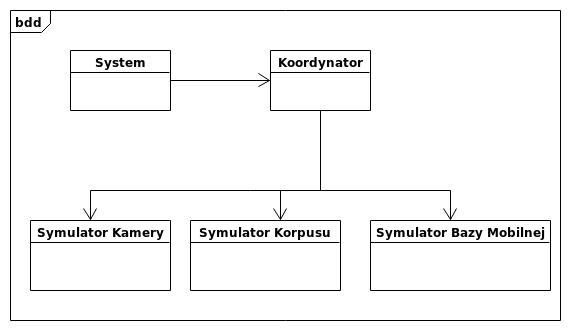
\includegraphics[scale=0.5]{./images/example_bdd.png}
        \caption{Poglądowa struktura systemu w SySML}
    \end{figure}
\end{frame}

%------------------------------------------------